\documentclass[12pt]{article}


% -------------------- PAQUETES --------------------
\usepackage[utf8]{inputenc}
\usepackage[spanish]{babel}
\usepackage[margin=2.54cm]{geometry}
\usepackage{graphicx}
\usepackage{xcolor}


% -------------------- CARGA DE ARCHIVOS EXTERNOS --------------------
% ----------------- UTILIDADES PARA DAR UN MEJOR FORMATO DE DOCUMENTO -----------------  


\definecolor{azul}{rgb}{0.0039, 0.3098, 0.6196}


% Formato para el indice general ...........
\makeatletter
    \renewcommand{\@dotsep}{1.5}
    \renewcommand{\l@section}{\@dottedtocline{1}{1.5em}{2.3em}}
    \renewcommand{\l@subsection}{\@dottedtocline{2}{3.8em}{3.2em}}
    \renewcommand{\l@subsubsection}{\@dottedtocline{3}{7.0em}{4.1em}}
\makeatother

% --------- COMANDOS PERSONALIZADOS PARA LA PORTADA DE LAS TAREAS, TRABAJOS Y PROYECTOS ---------

\newcommand{\rutaLogo}[1]{\newcommand{\RutaLogo}{#1}}
\newcommand{\tema}[1]{\newcommand{\Tema}{#1}}
\newcommand{\etiquetaAutores}[1]{\newcommand{\EtiquetaAutores}{#1}}
\newcommand{\alumno}[1]{\newcommand{\Alumno}{#1}}
\newcommand{\materia}[1]{\newcommand{\Materia}{#1}}
\newcommand{\docente}[1]{\newcommand{\Docente}{#1}}
\newcommand{\ciclo}[1]{\newcommand{\Ciclo}{#1}}
\newcommand{\fecha}[1]{\newcommand{\Fecha}{#1}}
\newcommand{\periodo}[1]{\newcommand{\Periodo}{#1}}



% -------------------- DEFINICIÓN DE LA PORTADA --------------------
\rutaLogo{../../../RecursosGlobales/Img/logo_tec_azuay.png}
\tema{\\ \vspace{1cm} Ejercicios propuestos sobre muestreo \\ \vspace{1.7cm}}
\etiquetaAutores{Alumno:}
\alumno{Eduardo Mendieta \vspace{1cm}}
\materia{Fundamentos de Estadística \vspace{1cm}}
\docente{Ing. Héctor Mejía, Mgtr. \vspace{1cm}}
\ciclo{Primer Ciclo - M1A \vspace{1.1cm}}
\fecha{18 de junio de 2024 \vspace{1cm}}
\periodo{Abril 2024 - Agosto 2024}



% -------------------- INFORME --------------------
\begin{document}

    \begin{titlepage}

    \centering

    \includegraphics[width=0.11\textwidth]{\RutaLogo} 

    \vspace{0.3cm}
    \textcolor{azul}{\Large \textbf{Instituto Superior Universitario Tecnológico del Azuay \\}}
    \vspace{0.3cm}
    \textcolor{azul}{\Large \textbf{Tecnología Superior en Big Data}}
    
    % 1. ---------------- TEMA -------------------------
    
    {\Large\textbf{\Tema}}
    
    % 2. ---------------- AUTOR(ES) -------------------------
    \textcolor{azul}{\large \textbf{\EtiquetaAutores} \\}
    \vspace{0.3cm}
    {\large \Alumno}

    % 3. ---------------- MATERIA -------------------------
    \textcolor{azul}{\large \textbf{Materia:} \\}
    \vspace{0.3cm}
    {\large \Materia}


    % 3. ---------------- DOCENTE -------------------------
    \textcolor{azul}{\large \textbf{Docente:} \\}
    \vspace{0.3cm}
    {\large \Docente}


    % 3. ---------------- Ciclo -------------------------
    \textcolor{azul}{\large \textbf{Ciclo:} \\}
    \vspace{0.3cm}
    {\large \Ciclo}


    % 3. ---------------- FECHA -------------------------
    \textcolor{azul}{\large \textbf{Fecha:} \\}
    \vspace{0.3cm}
    {\large \Fecha}

    % 3. ---------------- PERIODO -------------------------
    \textcolor{azul}{\large \textbf{Periodo Académico:} \\}
    \vspace{0.3cm}
    {\large \Periodo}
 
\end{titlepage}

  
    \section*{\centering Ejercicios propuestos}

        \vspace{0.6cm}
        \noindent \textbf{Resolver los ejercicios a mano y subir en un archivo  Pdf:}

        \vspace{0.6cm}
        \begin{itemize}
            \item \textbf{Ejercicio 1:} Un investigador desea estimar la proporción de estudiantes universitarios que utilizan el transporte público para ir a la universidad. Se desea una confianza del 95\% y un margen de error del 5\%. ¿Cuál es el tamaño de muestra necesario si se asume que la proporción esperada es del 50\%?
                \begin{figure}[!h]
                    \centering
                    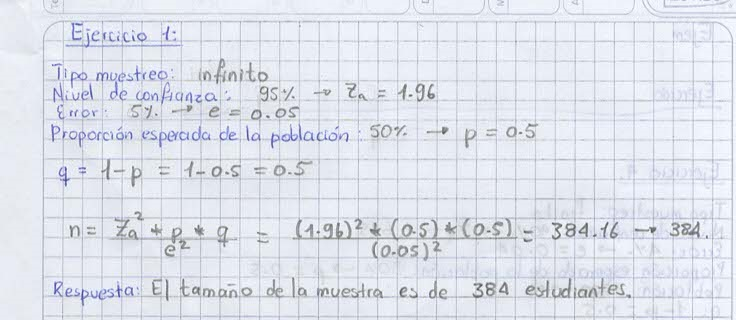
\includegraphics[width=0.9\textwidth]{Img/Tarea1_ej1.jpeg}
                \end{figure}
            
            \item \textbf{Ejercicio 2:} La empresa COLINEAL tiene 800 empleados y quiere realizar una encuesta sobre la satisfacción laboral. Se desea un nivel de confianza del 95\% y un margen de error del 5\%. ¿Cuál es el tamaño de la muestra necesario?
                \begin{figure}[!h]
                    \centering
                    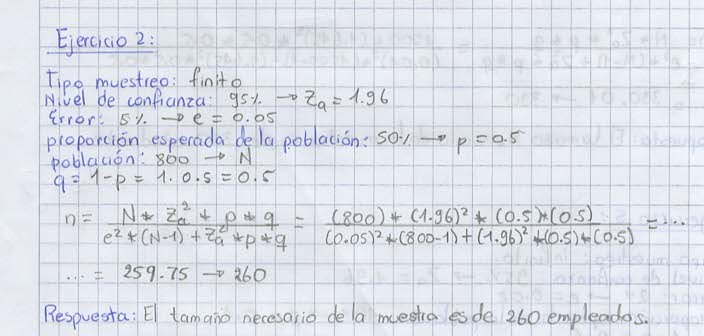
\includegraphics[width=0.9\textwidth]{Img/Tarea1_ej2.jpeg}
                \end{figure}
            
            \item \textbf{Ejercicio 3:} Una organización quiere estimar el porcentaje de hogares que tienen acceso a internet con una confianza del 99\% y un margen de error del 3\%. Si se asume que la proporción esperada es del 70\%, ¿cuál es el tamaño de la muestra necesario?
                \begin{figure}[!h]
                    \centering
                    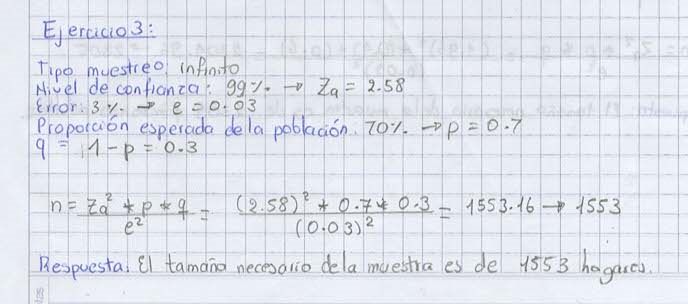
\includegraphics[width=0.9\textwidth]{Img/Tarea1_ej3.jpeg}
                \end{figure}
            
            \item \textbf{Ejercicio 4:} El ISTA tiene 1500 estudiantes y quiere hacer una encuesta sobre la satisfacción con las instalaciones deportivas. Se desea un nivel de confianza del 90\% y un margen de error del 4\%. ¿Cuál es el tamaño de la muestra necesario?
                \begin{figure}[!h]
                    \centering
                    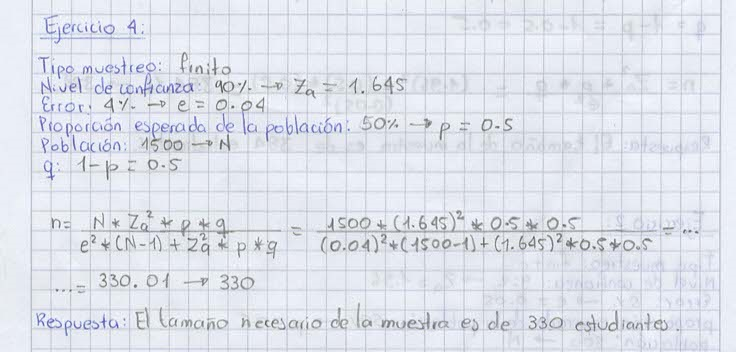
\includegraphics[width=0.9\textwidth]{Img/Tarea1_ej4.jpeg}
                \end{figure}
            
            \newpage
            \item \textbf{Ejercicio 5:} Un investigador está interesado en conocer la proporción de adultos que hacen ejercicio regularmente. Desea un nivel de confianza del 95\% y un margen de error del 2\%. ¿Cuál es el tamaño de la muestra necesario si se asume que la proporción esperada es del 40\%?
                \begin{figure}[!h]
                    \centering
                    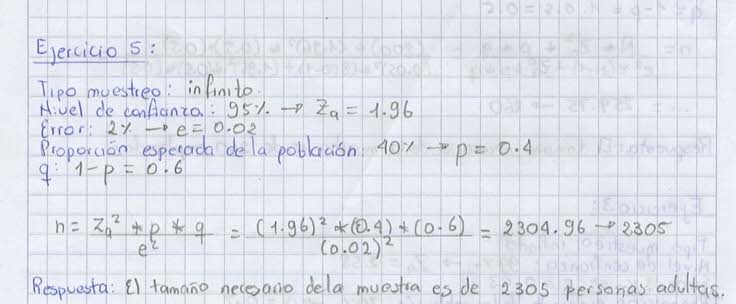
\includegraphics[width=0.9\textwidth]{Img/Tarea1_ej5.jpeg}
                \end{figure}
            
            \item \textbf{Ejercicio 6:} Una universidad tiene 3000 alumnos y desea realizar una encuesta para saber cuántos estudiantes están interesados en nuevos cursos de tecnología. Se desea un nivel de confianza del 95\% y un margen de error del 3\%. ¿Cuál es el tamaño de la muestra necesario?
                \begin{figure}[!h]
                    \centering
                    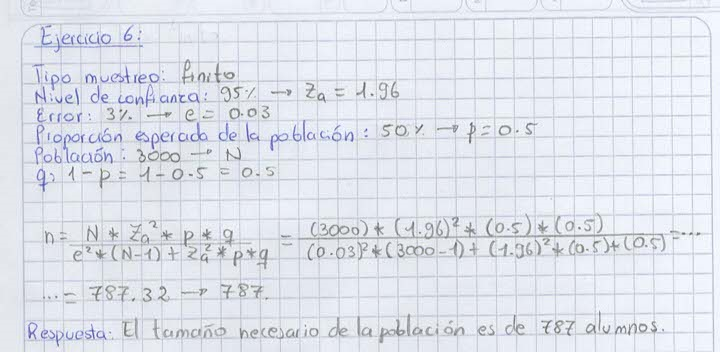
\includegraphics[width=0.9\textwidth]{Img/Tarea1_ej6.jpeg}
                \end{figure}

        \end{itemize}

\end{document}